%=====================================================================
\chapter{Résultats}\label{chap:res}
%=====================================================================
Sauf mention contraire, tous les résultats portent sur l'ensemble de \textbf{test} : 26 topologies jamais vues, 1\,042 simulations, 218\,628 flux dont 29\,851 en événement. Les métriques sont pondérées par flux. Le délai est exprimé en décades de log10 : une MAE de 0,175 correspond à une erreur multiplicative typique d'environ $\times1{,}5$.

\section{Entraînement du GNN}
\begin{figure}[H]
\centering
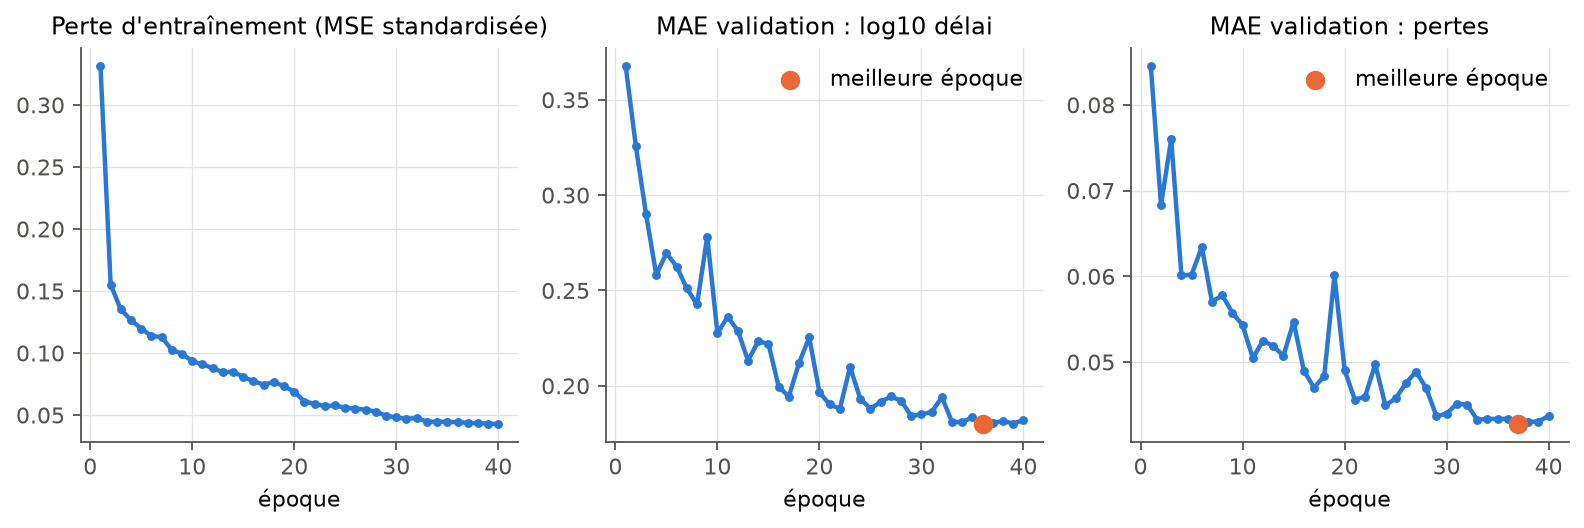
\includegraphics[width=\linewidth]{fig_training.png}
\caption{Courbes d'apprentissage du GNN : perte d'entraînement et MAE de validation (topologies inédites).}
\label{fig:training}
\end{figure}
La perte d'entraînement décroît régulièrement. La MAE de validation suit la même tendance, avec les oscillations attendues sur des topologies inédites, et atteint son minimum vers l'époque 36 (figure~\ref{fig:training}). On n'observe pas de divergence entre entraînement et validation, donc pas de surapprentissage marqué. La validation baisse encore légèrement à 40 époques : un entraînement plus long gagnerait probablement quelques centièmes. Trois initialisations donnent une MAE de test de 0,167 à 0,175 (écart-type de 0,004 décade).

\section{Comparaison globale et pendant les événements}
\begin{table}[H]
\centering\footnotesize
\adjustbox{max width=\linewidth}{\begin{tabular}{lrrrrrrr}
\toprule
Modèle & MAE global & MAE hors év. & MAE év. & MAE surch. & MAE délest. & MSE global & MSE év. \\
\midrule
Naïf & 0{,}825 & 0{,}686 & 1{,}707 & 1{,}723 & 1{,}644 & 1{,}286 & 4{,}612 \\
Ridge & 0{,}522 & 0{,}451 & 0{,}969 & 1{,}071 & 0{,}572 & 0{,}533 & 1{,}546 \\
Gradient Boosting & 0{,}276 & 0{,}215 & 0{,}664 & 0{,}749 & 0{,}335 & 0{,}311 & 1{,}130 \\
MLP & 0{,}343 & 0{,}286 & 0{,}705 & 0{,}797 & 0{,}344 & 0{,}362 & 1{,}211 \\
GNN & \textbf{0{,}175} & \textbf{0{,}159} & \textbf{0{,}271} & \textbf{0{,}312} & \textbf{0{,}111} & \textbf{0{,}140} & \textbf{0{,}255} \\
\bottomrule
\end{tabular}}
\caption{Cible log10(délai) : MAE et MSE (décades) sur le test, globalement et par sous-ensemble. En gras : le meilleur modèle.}
\label{tab:delai}
\end{table}
\begin{table}[H]
\centering\footnotesize
\adjustbox{max width=\linewidth}{\begin{tabular}{lrrrrrrr}
\toprule
Modèle & MAE global & MAE hors év. & MAE év. & MAE surch. & MAE délest. & MSE global & MSE év. \\
\midrule
Naïf & 0{,}196 & 0{,}153 & 0{,}472 & 0{,}549 & 0{,}173 & 0{,}089 & 0{,}314 \\
Ridge & 0{,}132 & 0{,}112 & 0{,}256 & 0{,}295 & 0{,}103 & 0{,}039 & 0{,}104 \\
Gradient Boosting & 0{,}067 & 0{,}053 & 0{,}154 & 0{,}186 & 0{,}028 & 0{,}020 & 0{,}066 \\
MLP & 0{,}082 & 0{,}067 & 0{,}173 & 0{,}207 & 0{,}041 & 0{,}023 & 0{,}076 \\
GNN & \textbf{0{,}045} & \textbf{0{,}039} & \textbf{0{,}078} & \textbf{0{,}095} & \textbf{0{,}010} & \textbf{0{,}010} & \textbf{0{,}024} \\
\bottomrule
\end{tabular}}
\caption{Cible taux de pertes : MAE et MSE sur le test.}
\label{tab:pertes}
\end{table}
\begin{figure}[H]
\centering
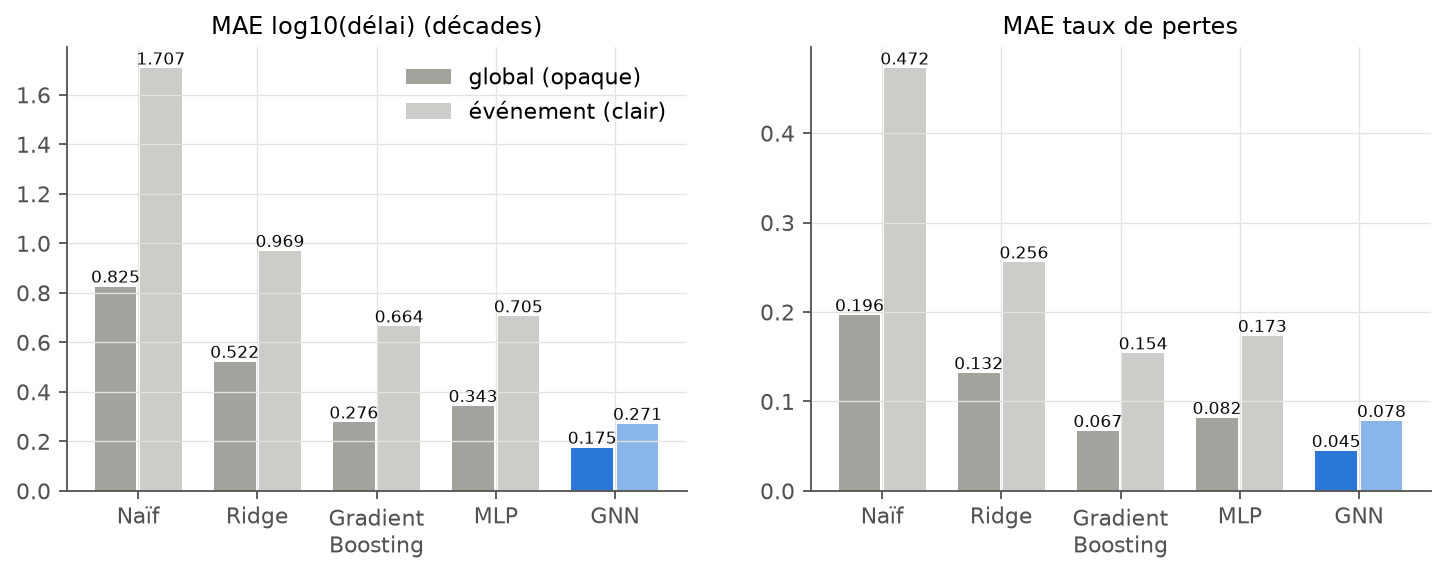
\includegraphics[width=\linewidth]{fig_comparison.png}
\caption{MAE globale (couleur pleine) et pendant les événements (couleur claire), pour les deux cibles.}
\label{fig:comparison}
\end{figure}

Les tableaux~\ref{tab:delai} et~\ref{tab:pertes} donnent un classement net et cohérent sur les deux cibles et les deux métriques.
\begin{itemize}
  \item \textbf{Naïf} (0,825 décade) et \textbf{Ridge} (0,522) restent loin derrière : la relation entre configuration et QoS est fortement non linéaire (coude en $b\approx1$).
  \item Le \textbf{Gradient Boosting} (0,276) est le meilleur modèle sans graphe, devant le \textbf{MLP} (0,343). Les deux voient exactement les mêmes 24 features.
  \item Le \textbf{GNN} réduit l'erreur de 37\,\% par rapport au Gradient Boosting (0,175) sur le délai, et de 33\,\% sur les pertes (0,045 contre 0,067). Sa MSE est 2,2 fois plus faible (0,140 contre 0,311) : il fait beaucoup moins de très grosses erreurs, ce que confirme la figure~\ref{fig:scatter}.
\end{itemize}

\paragraph{Pendant les événements.} Tous les modèles se dégradent, mais pas au même rythme.
\begin{itemize}
  \item La MAE du Gradient Boosting passe de 0,276 à 0,664 (×2,4), celle du MLP de 0,343 à 0,705, celle du GNN de 0,175 à 0,271 seulement (×1,55).
  \item En \textbf{surcharge}, le cas critique pour l'opérateur, le GNN se trompe de 0,31 décade, contre 0,75 pour le Gradient Boosting.
  \item En \textbf{délestage}, il reste au niveau du régime normal (0,11).
  \item Sur les pertes en événement, l'écart est d'un facteur 2 (0,078 contre 0,154).
\end{itemize}

\begin{figure}[H]
\centering
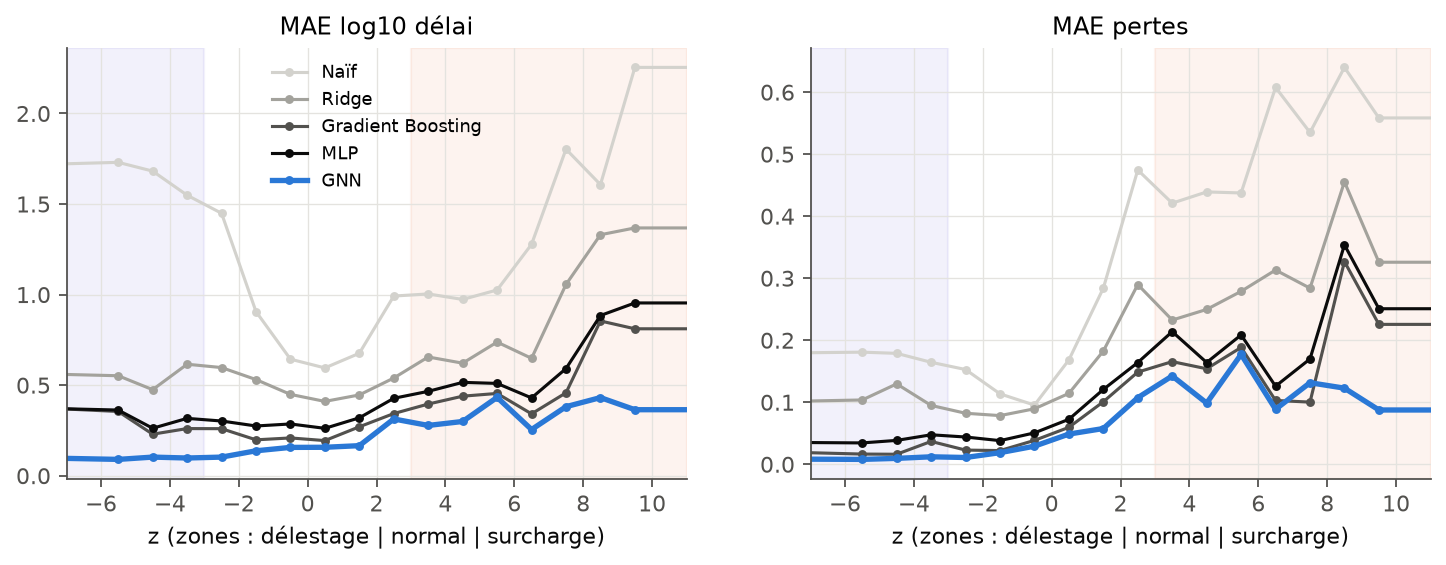
\includegraphics[width=\linewidth]{fig_errors_z.png}
\caption{MAE en fonction de l'écart $z$ au régime habituel (zones colorées : délestage à gauche, surcharge à droite).}
\label{fig:errors_z}
\end{figure}
La figure~\ref{fig:errors_z} montre la même chose en continu. Toutes les erreurs augmentent avec $z$ : plus la charge s'écarte du régime habituel, plus la prédiction est difficile, et l'hypothèse H2 est confirmée. C'est attendu : loin de la médiane, les configurations sont rares dans les données d'entraînement, et la QoS y est la plus sensible à la charge (zone de saturation, section~\ref{sec:sota-alloc}). La pente est cependant beaucoup plus faible pour le GNN. Côté délestage, son erreur ne bouge presque pas, alors que celle des modèles tabulaires remonte.

\begin{figure}[H]
\centering
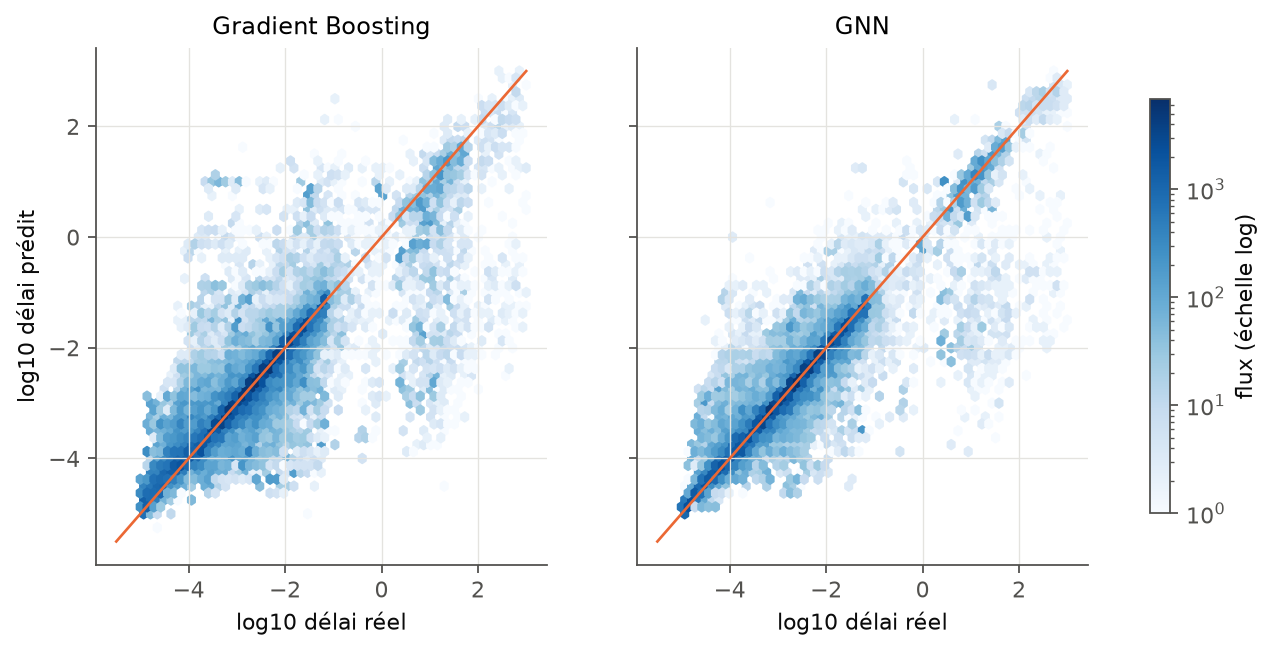
\includegraphics[width=0.85\linewidth]{fig_scatter.png}
\caption{Délai prédit contre délai réel (test, densité de flux en échelle log) : Gradient Boosting et GNN.}
\label{fig:scatter}
\end{figure}
Sur la figure~\ref{fig:scatter}, le nuage du Gradient Boosting présente des bandes horizontales et verticales : il confond les régimes congestionné et non congestionné. Le GNN se concentre beaucoup plus autour de la diagonale, y compris pour les délais extrêmes des files affamées (au-delà de 1~s).

\section{Par type de slice}
\begin{table}[H]
\centering\footnotesize
\adjustbox{max width=\linewidth}{\begin{tabular}{lrrrrrr}
\toprule
Modèle & MAE délai URLLC & MAE délai eMBB & MAE délai mMTC & MAE pertes URLLC & MAE pertes eMBB & MAE pertes mMTC \\
\midrule
Naïf & 0{,}753 & 0{,}654 & 0{,}857 & 0{,}217 & 0{,}208 & 0{,}190 \\
Ridge & 0{,}506 & 0{,}575 & 0{,}523 & 0{,}136 & 0{,}149 & 0{,}129 \\
Gradient Boosting & 0{,}246 & 0{,}340 & 0{,}282 & 0{,}058 & 0{,}092 & 0{,}068 \\
MLP & 0{,}305 & 0{,}382 & 0{,}352 & 0{,}070 & 0{,}105 & 0{,}083 \\
GNN & \textbf{0{,}194} & \textbf{0{,}257} & \textbf{0{,}164} & \textbf{0{,}047} & \textbf{0{,}071} & \textbf{0{,}042} \\
\bottomrule
\end{tabular}}
\caption{MAE par type de slice (test).}
\label{tab:slice}
\end{table}
Le classement est le même pour les trois slices (tableau~\ref{tab:slice}). eMBB est la plus difficile pour tous les modèles appris : peu de flux, de gros paquets, des files très sensibles à leur poids. C'est sur mMTC que le GNN gagne le plus : 0,164 contre 0,282. Les flux mMTC sont nombreux et petits, et leur QoS dépend surtout de la congestion créée par les autres slices sur les liens partagés.

\section{Utilité opérationnelle : détection des violations de SLA}
\begin{table}[H]
\centering\footnotesize
\adjustbox{max width=\linewidth}{\begin{tabular}{lrrrr}
\toprule
Modèle & Exact. équil. global & Exact. équil. événement & F1 violation global & F1 violation événement \\
\midrule
Naïf & 0{,}500 & 0{,}500 & 0{,}690 & 0{,}874 \\
Ridge & 0{,}765 & 0{,}746 & 0{,}778 & 0{,}905 \\
Gradient Boosting & 0{,}907 & 0{,}836 & 0{,}912 & 0{,}941 \\
MLP & 0{,}871 & 0{,}830 & 0{,}874 & 0{,}936 \\
GNN & \textbf{0{,}926} & \textbf{0{,}858} & \textbf{0{,}929} & \textbf{0{,}944} \\
\bottomrule
\end{tabular}}
\caption{Décision « délai prédit au-dessus du SLA ? » pour eMBB (10~ms) et URLLC (0,5~ms) : exactitude équilibrée et F1 de la classe « violation ».}
\label{tab:sla}
\end{table}
Transformée en décision binaire, la prédiction reste utile (tableau~\ref{tab:sla}). Le GNN atteint une exactitude équilibrée de 0,926 (0,858 pendant les événements), contre 0,907 (0,836) pour le Gradient Boosting et 0,500 pour le modèle naïf. L'écart est plus faible que sur la MAE : un flux loin du seuil est bien classé par tous les modèles non linéaires. Le gain du GNN porte surtout sur les flux proches du seuil et sur l'\emph{ampleur} des dégradations, qui compte pour choisir de combien augmenter une réservation.

\section{Ablation}
\begin{table}[H]
\centering\footnotesize
\adjustbox{max width=\linewidth}{\begin{tabular}{llrrrr}
\toprule
Modèle & Variante & MAE délai & Δ MAE délai & MAE pertes & Δ MAE pertes \\
\midrule
Ridge & complet & 0{,}522 & 0{,}000 & 0{,}132 & 0{,}000 \\
Ridge & sans réservation & 0{,}553 & 0{,}031 & 0{,}140 & 0{,}008 \\
Ridge & sans charge & 0{,}556 & 0{,}034 & 0{,}176 & 0{,}045 \\
Ridge & sans physique & 0{,}605 & 0{,}084 & 0{,}133 & 0{,}001 \\
Ridge & sans allocation & 0{,}605 & 0{,}083 & 0{,}154 & 0{,}022 \\
Gradient Boosting & complet & 0{,}276 & 0{,}000 & 0{,}067 & 0{,}000 \\
Gradient Boosting & sans réservation & 0{,}314 & 0{,}037 & 0{,}077 & 0{,}010 \\
Gradient Boosting & sans charge & 0{,}429 & 0{,}153 & 0{,}152 & 0{,}085 \\
Gradient Boosting & sans physique & 0{,}279 & 0{,}002 & 0{,}068 & 0{,}001 \\
Gradient Boosting & sans allocation & 0{,}453 & 0{,}176 & 0{,}128 & 0{,}061 \\
MLP & complet & 0{,}343 & 0{,}000 & 0{,}082 & 0{,}000 \\
MLP & sans réservation & 0{,}361 & 0{,}018 & 0{,}092 & 0{,}010 \\
MLP & sans charge & 0{,}448 & 0{,}105 & 0{,}154 & 0{,}073 \\
MLP & sans physique & 0{,}367 & 0{,}024 & 0{,}094 & 0{,}013 \\
MLP & sans allocation & 0{,}469 & 0{,}126 & 0{,}129 & 0{,}048 \\
GNN & complet & 0{,}175 & 0{,}000 & 0{,}045 & 0{,}000 \\
GNN & sans réservation & 0{,}179 & 0{,}004 & 0{,}046 & 0{,}001 \\
GNN & sans charge & 0{,}367 & 0{,}192 & 0{,}120 & 0{,}075 \\
GNN & sans physique & 0{,}182 & 0{,}008 & 0{,}043 & -0{,}002 \\
GNN & sans allocation & 0{,}402 & 0{,}227 & 0{,}114 & 0{,}069 \\
GNN & T = 0 (sans interactions) & 0{,}240 & 0{,}065 & 0{,}062 & 0{,}017 \\
GNN & sans nœuds file & 0{,}428 & 0{,}254 & 0{,}098 & 0{,}053 \\
\bottomrule
\end{tabular}}
\caption{Ablation (test) : MAE après retrait d'une famille de features, ou d'un élément de structure du GNN, et écart avec le modèle complet.}
\label{tab:ablation}
\end{table}
\begin{figure}[H]
\centering
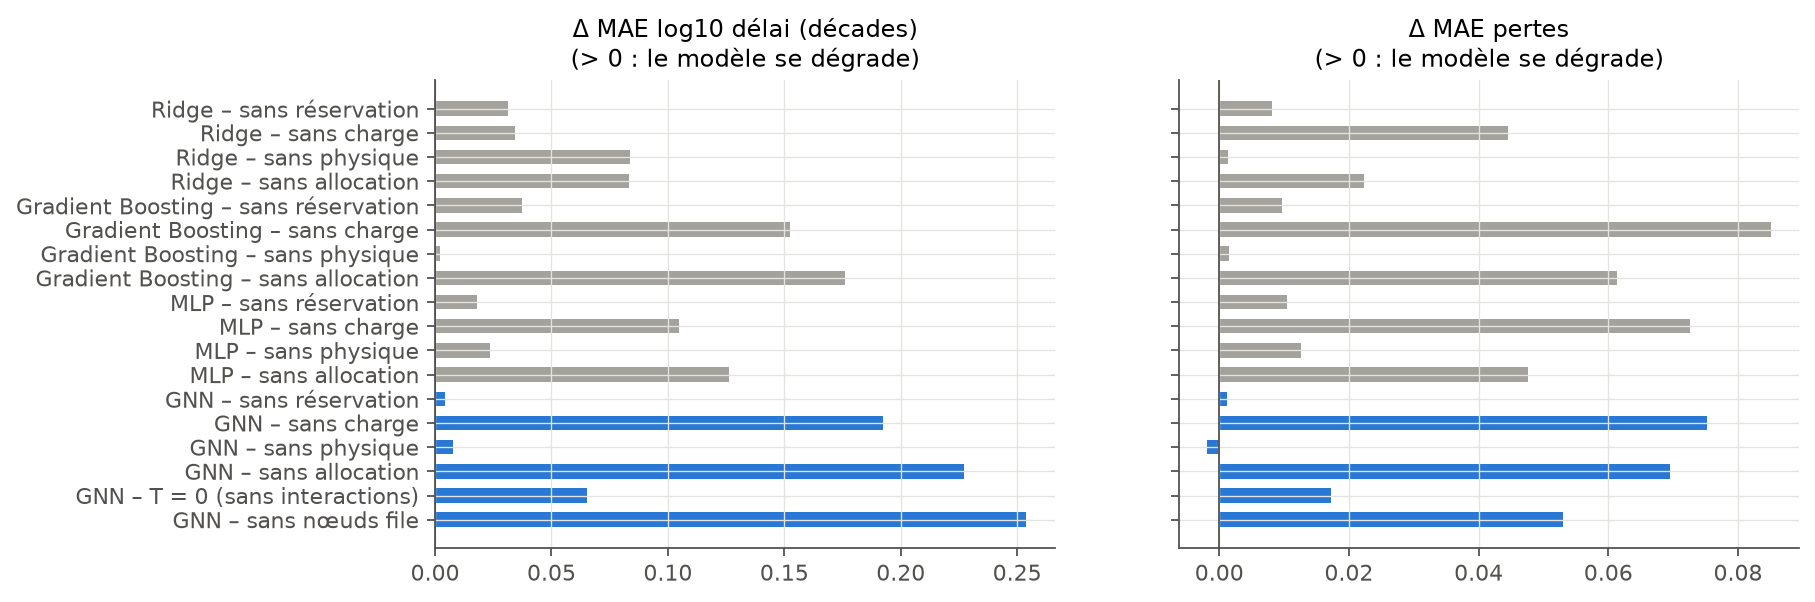
\includegraphics[width=\linewidth]{fig_ablation.png}
\caption{Hausse de la MAE après chaque ablation (en bleu : GNN).}
\label{fig:ablation}
\end{figure}
Le tableau~\ref{tab:ablation} et la figure~\ref{fig:ablation} répondent à trois questions.

\paragraph{D'où vient le gain du GNN ?}
\begin{itemize}
  \item Avec $T=0$, chaque flux ne lit qu'une fois l'état initial des liens et des files : pas de rétroaction, donc pas d'interaction entre flux. La MAE remonte alors à 0,240, et à 0,502 pendant les événements. Les interactions expliquent donc environ 60\,\% de l'écart avec le Gradient Boosting, globalement (0,065 sur 0,101 décade) comme pendant les événements (0,231 sur 0,393) : c'est l'hypothèse H1.
  \item Sans nœuds « file WFQ », le GNN tombe à 0,428, moins bon que le Gradient Boosting. La représentation explicite des réservations par slice est indispensable.
\end{itemize}

\paragraph{Quelles informations sont nécessaires ?} Retirer toute l'information d'\emph{allocation} ($\delta$, poids, débit réservé, délai de file pleine) fait passer le GNN de 0,175 à 0,402 (0,94 pendant les événements) et le Gradient Boosting de 0,276 à 0,453. Retirer la \emph{charge} coûte presque autant : 0,367 pour le GNN. Les deux familles sont nécessaires, ce qui confirme l'hypothèse H3. Les familles « réservation » et « physique » sont en revanche redondantes : le délai de file pleine dépend du débit WFQ effectif, donc du poids. Retirer l'une sans l'autre ne coûte presque rien, d'où la variante « allocation » qui retire les deux.

\paragraph{La connaissance du domaine aide-t-elle ?} La feature physique (délai de file pleine) est la plus importante pour le Gradient Boosting (figure~\ref{fig:importance}). Elle améliore nettement Ridge : 0,605 sans elle, 0,522 avec. Elle n'apporte presque rien au GNN (0,182 sans, 0,175 avec), qui reconstruit cette relation à partir des poids, des capacités et des tailles de paquets.

\begin{figure}[H]
\centering
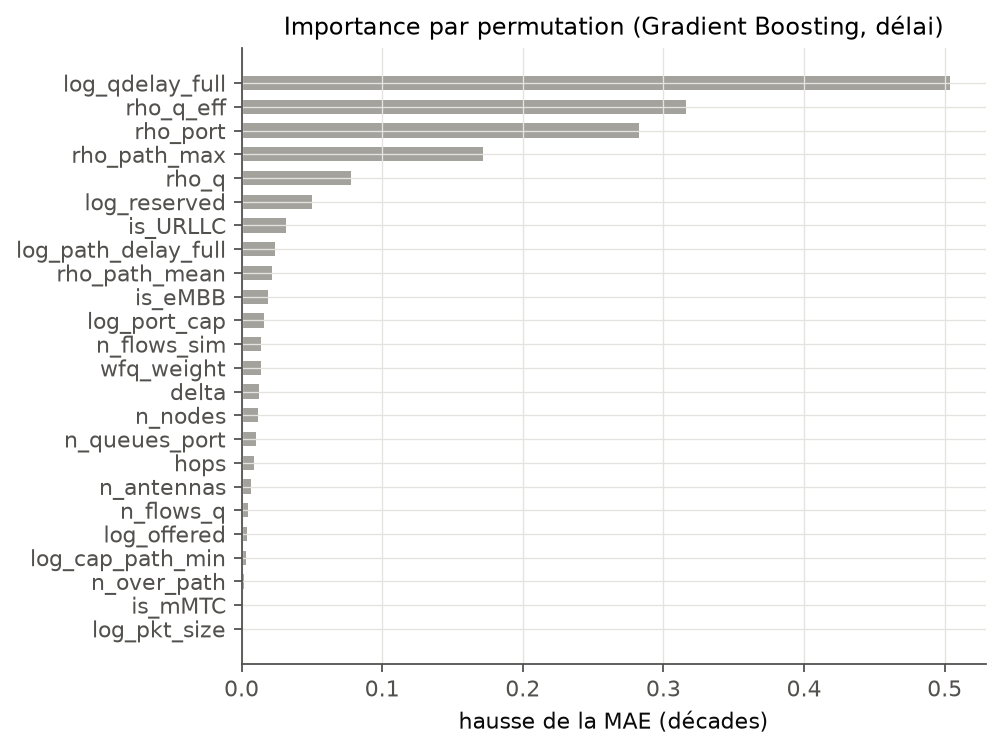
\includegraphics[width=0.62\linewidth]{fig_importance.png}
\caption{Importance par permutation~\cite{breiman} des features du Gradient Boosting (cible délai, test) : hausse de la MAE quand on mélange une feature.}
\label{fig:importance}
\end{figure}

\section{Décalage de distribution : grands réseaux}
\begin{table}[H]
\centering\footnotesize
\adjustbox{max width=\linewidth}{\begin{tabular}{lrrrrr}
\toprule
Modèle & MAE délai (topo) & MAE délai (grands) & MAE pertes (topo) & MAE pertes (grands) & MAE délai (grands, év.) \\
\midrule
Naïf & 0{,}825 & 0{,}840 & 0{,}196 & 0{,}206 & 1{,}556 \\
Ridge & 0{,}522 & 0{,}552 & 0{,}132 & 0{,}139 & 0{,}837 \\
Gradient Boosting & 0{,}276 & 0{,}293 & 0{,}067 & 0{,}075 & 0{,}573 \\
MLP & 0{,}343 & 0{,}361 & 0{,}082 & 0{,}091 & 0{,}600 \\
GNN & \textbf{0{,}175} & \textbf{0{,}203} & \textbf{0{,}045} & \textbf{0{,}053} & \textbf{0{,}283} \\
\bottomrule
\end{tabular}}
\caption{MAE sur le test du découpage aléatoire (« topo ») et sur le test des grands réseaux (« grands », topologies de 212 nœuds et plus, absentes de l'entraînement).}
\label{tab:shift}
\end{table}
\begin{figure}[H]
\centering
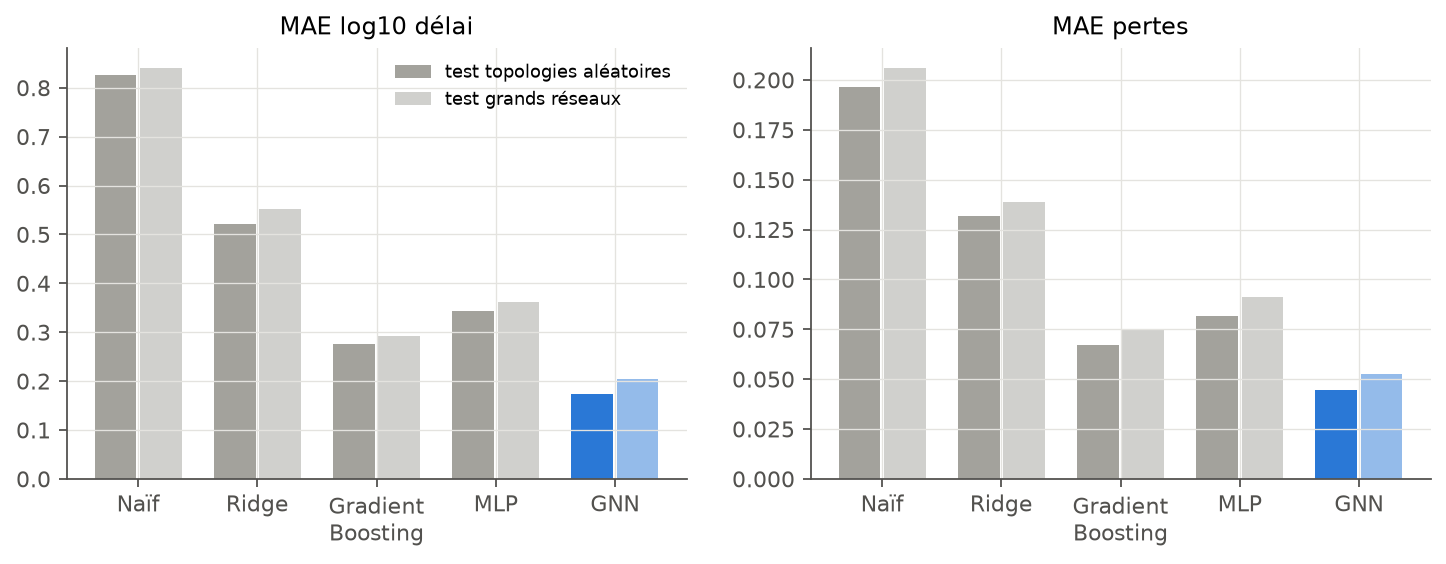
\includegraphics[width=\linewidth]{fig_shift.png}
\caption{Effet du décalage de distribution sur la taille des réseaux.}
\label{fig:shift}
\end{figure}
Entraînés sur les petits et moyens réseaux puis testés sur les plus grands, tous les modèles se dégradent un peu (tableau~\ref{tab:shift}). C'est un décalage de covariables~\cite{datasetshift} : la loi des entrées change (chemins plus longs, liens plus partagés), pas la physique qui relie entrées et QoS.
\begin{itemize}
  \item Le GNN passe de 0,175 à 0,203 (+16\,\%), le Gradient Boosting de 0,276 à 0,293 (+6\,\%).
  \item Le GNN reste nettement le meilleur, y compris pendant les événements de ces grands réseaux : 0,283 contre 0,573.
  \item Sa dégradation relative plus forte rappelle qu'un GNN généralise à des tailles nouvelles sans garantie : les chemins plus longs et les liens plus partagés sortent de ce qu'il a vu. Il n'a en revanche besoin d'aucune adaptation pour s'appliquer à un graphe plus grand.
\end{itemize}

%=====================================================================
\chapter{Discussion}\label{chap:disc}
%=====================================================================
\section{Réponses aux questions d'analyse du guide}
\begin{description}
  \item[Quel modèle généralise le mieux ?] Le GNN, sur des topologies jamais vues (MAE de 0,175 décade sur le délai et de 0,045 sur les pertes) comme sur des réseaux plus grands que ceux de l'entraînement (0,203). L'écart avec le Gradient Boosting est environ 25 fois plus grand que la variabilité due à l'initialisation.
  \item[Quel modèle résiste le mieux aux événements ?] Le GNN : son erreur n'augmente que de 55\,\% pendant les événements, contre 140\,\% pour le Gradient Boosting. En surcharge, il est 2,4 fois plus précis.
  \item[Le GNN apporte-t-il un gain réel ?] Oui : $-37\,\%$ de MAE globalement et $-59\,\%$ pendant les événements, avec une cause identifiée par l'ablation (interactions entre flux et files WFQ explicites). En décision SLA binaire, le gain est réel mais plus modeste (+0,02 d'exactitude équilibrée).
  \item[Quelles features sont importantes ?] L'allocation (poids WFQ et grandeurs qui en dérivent) et la charge des files, du port et des liens. La structure de la topologie seule et le type de slice comptent peu. Pour les modèles sans graphe, le délai de file pleine, une connaissance du domaine, est la feature dominante.
  \item[Les performances changent-elles quand la distribution diffère ?] Oui, modérément : de +2 à +16\,\% d'erreur sur les grands réseaux selon le modèle, sans changement de classement.
  \item[Quelles sont les limites ?] Voir la section~\ref{sec:limites}.
\end{description}

\section{« Meilleur score » ne veut pas dire « meilleure solution »}
Le GNN a le meilleur score, mais son coût est plus élevé. Il faut environ 16~minutes d'entraînement sur GPU (cinq fois plus sur CPU), contre 2~minutes pour le Gradient Boosting. Il demande aussi de construire un graphe par configuration et il est plus difficile à expliquer. Pour un contrôle d'admission grossier, loin des seuils, un Gradient Boosting bien alimenté en features physiques donne déjà 0,907 d'exactitude équilibrée. Le GNN se justifie quand on a besoin de l'\emph{ampleur} des dégradations et d'une fiabilité dans les situations inhabituelles, c'est-à-dire pour la gestion \emph{dynamique} des slices.

\section{Trois choix méthodologiques défendus}
\begin{enumerate}
  \item \textbf{Vérifier les entrées contre les sorties avant de modéliser.} Confronter la charge offerte calculée à l'utilisation mesurée a révélé que 42\,\% des chemins du fichier de slices étaient faux. Sans cette vérification, tous les modèles auraient appris sur des entrées erronées, sans aucun message d'erreur. La qualité des données a ici pesé plus lourd que le choix du modèle.
  \item \textbf{Découper par topologie et évaluer par flux.} Le découpage par topologie empêche de mémoriser un réseau. Les classes de flux pondérées rendent le calcul six fois plus léger sans changer une seule métrique.
  \item \textbf{Définir les événements sur les entrées, en log, avec une règle robuste.} Le masque est observable par l'opérateur avant toute mesure, il ne dépend pas de la cible (pas de biais de sélection) et il est cohérent avec la physique du problème : coude en $b\approx1$, écarts multiplicatifs, queues lourdes d'où la règle de Hampel.
\end{enumerate}

\section{Limites}\label{sec:limites}
\begin{itemize}
  \item \textbf{Un seul simulateur}, des régimes stationnaires et un réseau de transport filaire sans partie radio : les conclusions valent pour ce cadre.
  \item \textbf{Événements reconstruits} : faute d'axe temporel, un événement est un écart au régime habituel de la topologie, pas une transition observée. Le comportement \emph{pendant} la transition (régime transitoire) n'est pas étudié.
  \item \textbf{Défauts du dataset} : une partie des surcharges vient des réservations hors chemin. Elles sont réelles dans les simulations, mais un opérateur ne les produirait probablement pas volontairement.
  \item \textbf{Variabilité} estimée seulement sur l'initialisation du GNN (3 graines), pas sur la découpe des topologies ; hyperparamètres du GNN non optimisés ; entraînement arrêté à 40 époques alors que la validation baissait encore légèrement.
  \item \textbf{Prédiction et non décision} : le modèle évalue une allocation, il ne choisit pas $\delta$. Une boucle d'optimisation (recherche des poids minimaux respectant les SLA) reste à construire.
\end{itemize}

%=====================================================================
\chapter{Conclusion}\label{chap:concl}
%=====================================================================
Nous avons construit un jumeau numérique de la QoS des slices à partir du dataset \emph{B5G Network Slicing}. Il prédit le délai et les pertes de chaque flux à partir de la configuration du réseau et des réservations WFQ. Après correction de plusieurs défauts du dataset, un GNN hétérogène flux / files WFQ / liens prédit le délai avec une erreur typique d'un facteur 1,5. Il réduit l'erreur de 37\,\% par rapport au meilleur modèle sans graphe, et de 59\,\% pendant les changements brusques du réseau, là où les modèles tabulaires se dégradent le plus.

\paragraph{Réponse à la question finale.} \emph{Dans quelles conditions une approche GNN apporte-t-elle une valeur ajoutée pour la gestion dynamique des slices B5G ?} Nos expériences en identifient quatre :
\begin{enumerate}
  \item \textbf{quand la QoS dépend de ressources partagées et d'effets en cascade} (congestion des liens communs, pertes en amont) que des features par flux ne peuvent pas résumer. L'ablation $T=0$ montre que la rétroaction flux $\leftrightarrow$ liens est la source principale du gain ;
  \item \textbf{quand le graphe représente explicitement le levier de gestion}, ici les files WFQ par slice. Un GNN qui ne les voit pas perd tout son avantage ;
  \item \textbf{quand le réseau sort de son régime habituel} (surcharges, délestages). C'est le cas d'usage de la gestion dynamique, et c'est là que l'écart avec les modèles tabulaires est le plus grand ;
  \item \textbf{quand la topologie change ou grandit} : le même modèle s'applique à des réseaux inédits, avec une dégradation modérée.
\end{enumerate}
À l'inverse, pour des décisions grossières loin des seuils, ou quand le coût d'entraînement compte, un Gradient Boosting nourri de features physiques reste une alternative solide. L'étape suivante consiste à boucler le jumeau numérique avec un optimiseur des réservations $\delta$, et à le valider sur des traces temporelles réelles.
